\subsubsection{2.2. Đồ thị đa quan hệ nhận thức ràng buộc (Constraint-Aware Graph)}

\indent\indent Trong môi trường mạng xã hội phi tập trung (DeSo), dữ liệu không chỉ mang tính phi cấu trúc mà còn tiềm ẩn những mối quan hệ ràng buộc phức tạp trên chuỗi khối (\textit{on-chain}). Để nhận diện hiệu quả các thực thể Sybil vốn có khả năng ngụy tạo hành vi tinh vi, nghiên cứu đề xuất chuyển đổi dữ liệu thô thành cấu trúc \textbf{Đồ thị đa quan hệ nhận thức ràng buộc} (\textit{Constraint-Aware Multi-relational Graph}).\vspace{0.3cm}

Việc sử dụng đồ thị đa quan hệ là yếu tố then chốt để bảo tồn ngữ cảnh hành vi. Theo Akoglu và cộng sự \cite{akoglu2015graph}, các thực thể độc hại có thể dễ dàng ngụy tạo các kết nối đơn lẻ, nhưng rất khó để bắt chước toàn bộ hệ sinh thái ràng buộc đa tầng của một người dùng thực mà không để lại các mẫu dị thường về mặt cấu trúc.

\begin{figure}[H]
    \centering
    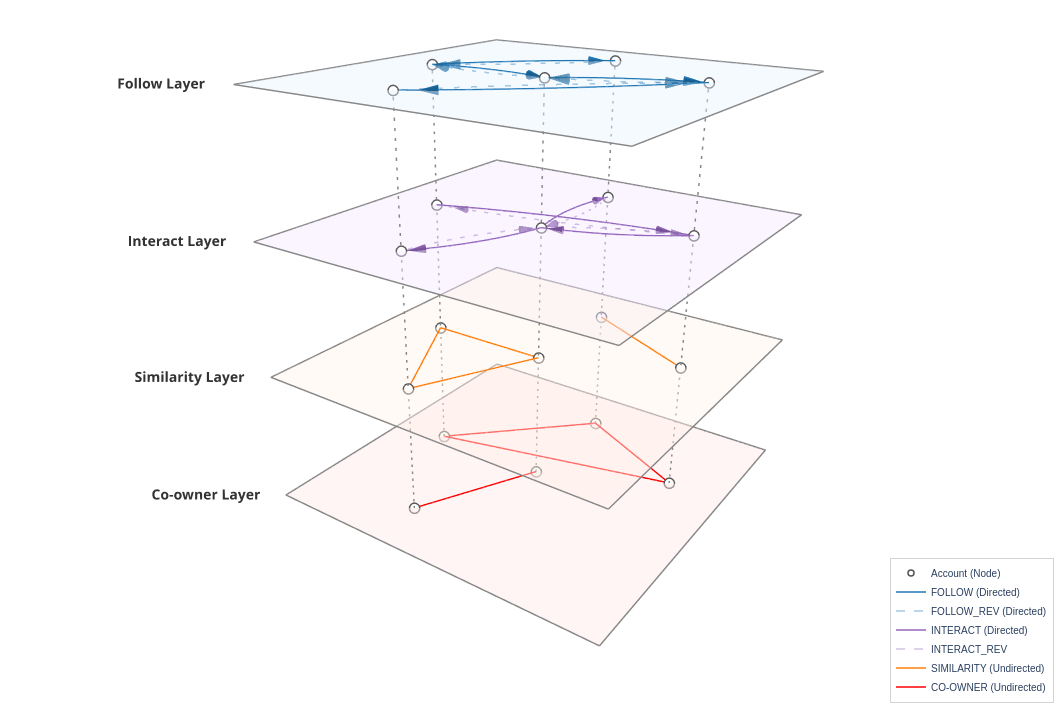
\includegraphics[width=1\linewidth]{images/part-02/chap-01/MLG.png}
    \caption{Kiến trúc Đồ thị đa quan hệ nhận thức ràng buộc trong hệ thống SybilSignal}
    \label{fig:MRG}
\end{figure}

Giải pháp của đề tài thiết lập 4 tầng quan hệ chiến lược. Mỗi tầng phản ánh một khía cạnh hành vi khác nhau với mức độ tin cậy được định lượng hóa thông qua các trọng số cơ sở ($W_{base}$):\vspace{-0.1cm}

\begin{itemize}[label={--}, itemsep=3pt]
    \item \textbf{Tầng Theo dõi ($W_{base} = 1$):} Phản ánh các kết nối xã hội cơ bản. Tầng này được gán trọng số thấp nhất do chi phí thực hiện hành vi theo dõi là tối thiểu. Các mạng lưới Sybil thường lợi dụng đặc điểm này để thực hiện "theo dõi chéo", dẫn đến nhiễu cao.
    
    \item \textbf{Tầng Tương tác ($W_{base} = 2$):} Bao gồm các hành vi trao đổi thông tin và giá trị thực (như yêu thích, bình luận, chia sẻ bài viết). Trọng số gấp đôi so với tầng theo dõi do các hành vi này đòi hỏi hao phí về phí giao dịch.

    \item \textbf{Tầng Tương đồng ($W_{base} = 5$):} Tầng này được thiết kế chuyên biệt để bóc tách đặc tính "sản xuất hàng loạt" của hệ thống Sybil. Cạnh tương đồng được thiết lập chặt chẽ thông qua nguyên tắc \textbf{ràng buộc 2/3}: hai tài khoản phải chia sẻ ít nhất hai trong ba dấu hiệu dị thường gồm: (1) tương đồng cao về ngữ nghĩa tiểu sử, (2) khoảng cách chỉnh sửa tên định danh (\textit{Normalized Levenshtein Distance}) \cite{yujian2007normalized} rất hẹp, và (3) sự hội tụ về thời gian khởi tạo. Trọng số mức 5 đóng vai trò như một lực liên kết mạnh, chủ động gom cụm các tài khoản bị nghi ngờ sinh ra từ cùng một kịch bản tự động.
    
    \item \textbf{Tầng Đồng sở hữu ($W_{base} = 10$):} Là tầng mang tính quyết định với trọng số tuyệt đối. Trong mạng xã hội phi tập trung, việc nhiều hồ sơ mạng xã hội được quản lý bởi chung một địa chỉ ví mã hóa là minh chứng kỹ thuật về tính sở hữu trên nền tảng.
\end{itemize}

Một thách thức kinh điển trong khai phá đồ thị mạng xã hội là sự tồn tại của các nút siêu đặc. Nếu duy trì tần suất tương tác dưới dạng tuyến tính, tín hiệu từ các nút siêu đặc này sẽ áp đảo quá trình truyền thông điệp, gây ra hiện tượng quá mịn làm mờ đi các cấu trúc Sybil cục bộ.\vspace{0.3cm}

Để giải quyết vấn đề này, đề tài áp dụng cơ chế \textbf{chuẩn hóa logarit phi tuyến} cho trọng số cạnh cuối cùng:
\[
    W_{final} = W_{base} \times \log_{10}(1 + \text{count})
\]

Trong đó, \textit{count} là tần suất thực hiện hành vi. Lấy cảm hứng từ cơ chế \textit{logarithmic scalers} trong kiến trúc mạng PNA \cite{corso2020principal}, hàm chuẩn hóa này giúp nén biên độ của các ngoại lệ thống kê. Nó đảm bảo hệ thống vừa đánh giá cao các liên kết lặp lại nhiều lần, vừa ngăn chặn sự thống trị của các luồng tương tác quy mô lớn, từ đó tối ưu hóa khả năng trích xuất đặc trưng của mạng GNN.